\lesson{Collision Theory}
Collision theory helps explain the reaction rates of different reactions. According to collision
theory, chemical reactions can only occur if energy is provided to break those bonds, the source
of that energy being the kinetic energy of molecules.

\begin{definition}{Concepts of Collision Theory}
    \begin{bulleted-list}
        \item A chemical reaction must involve \textit{collisions of particles} which each other
            and the walls of the container
        \item An \textbf{effective collision} is one that has sufficient energy and correct
            orientation of the colliding particles so that bonds can be broken and new bonds form
            (Figure \ref{fig:orientation-of-colliding-molecules})
        \item \textbf{Ineffective collisions} involve particles that rebound from the collision,
            essentially unchanged in nature
        \item The rate of a given reaction depends on the \textit{frequency of collisions} and the
            \textit{fraction} of those collisions that are effective
    \end{bulleted-list}
\end{definition}

\begin{figure}[ht!]
    \centering
    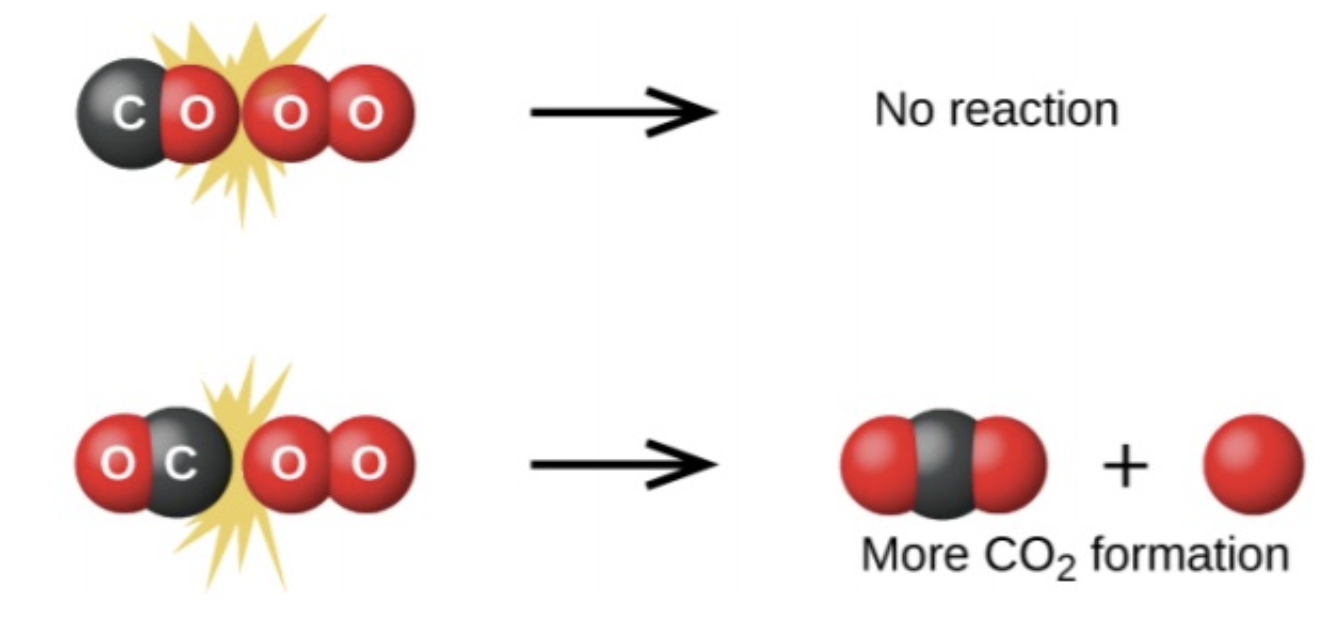
\includegraphics[width=0.6 \textwidth]{../figures/orientation of colliding molecules.png}
    \caption{Orieentation of colliding molecules}
    \label{fig:orientation-of-colliding-molecules}
\end{figure}

The formula for the rate in terms of the frequency collisions and fraction of effective collisions is
\[
    \text{rate}=(\text{frequency of collisions})\times(\text{fraction of effective collisions})
\]
For instance, consider the rate when the frequency of collisions is 1000 collisions per second and
the fraction of effective collisions is 1 in 100, the reaction rate is
\begin{align*}
    \text{rate}&=(\text{frequency of collisions})\times(\text{fraction of effective collisions})\\
               &=\frac{1000\,\si{collisions}}{1\,\si{s}}\times\frac{1\,\si{reaction}}{100\,\si{collisions}}\\
               &=10\,\frac{\text{reactions}}{\text{s}}
\end{align*}

\subsection{Activation Energy}
Activation energy, denoted by $E_\text{act}$, is the minimum increase in potential energy of a 
system required for molecules to react. See Figure \ref{fig:activation-energy}. Once the activation
energy is reached for a reaction, the kinetic energy is either converted into potential energy
in an endothermic reaction or potential energy is converted into kinetic energy in an exothermic
reaction. Keep in mind that temperature is a measure of the \textbf{average kinetic energy} in
a system.\\

For instance, for the sulfur tip of a match, it is particularly easy to create an ignition reaction.
However, on the wood end, it requires much more energy to create a reaction. This implies that
the sulfur has a lower activation energy compared to wood.

\begin{important}
    In an exothermic reaction, kinetic energy (measured by temperature) is released into the
    surroundings, which would increase the kinetic energy of neighbouring molecules and thus cause
    more exothermic reactions. Consequently, a positive feedback loop is achived. An example of
    this is can be seen in a wildfire, where the kinetic energy released causes the fire to grow.
    Increasing temperature has a particular dramatic effect on the reaction rate because it
    increases both collision frequency and the fraction of effective collisions (due to increase
    in kinetic energy).
\end{important}

\begin{important}
    Any reaction, exothermic or endothermic, requires an initial investment of energy; namely,
    \textbf{activation energy}.
\end{important}

\begin{figure}[ht!]
    \centering
    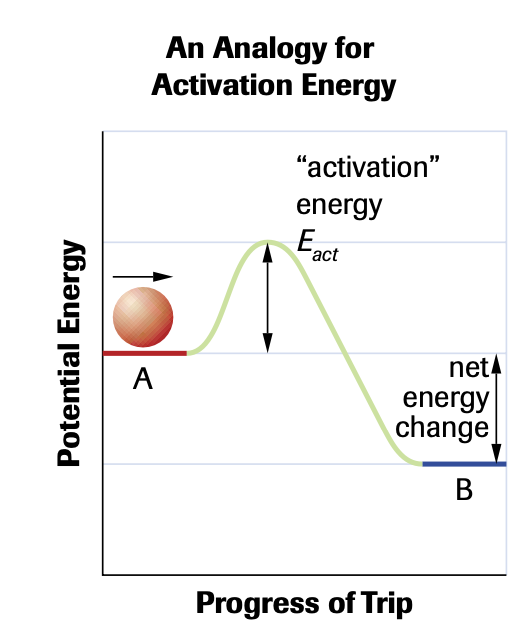
\includegraphics[width=0.5 \textwidth]{../figures/activation energy.png}
    \caption{The activation is required to start the reaction. This figure demonstrates an
        exothermic reaction, since the products have less potential energy than the reactants.}
    \label{fig:activation-energy}
\end{figure}

\begin{figure}[ht!]
    \centering
    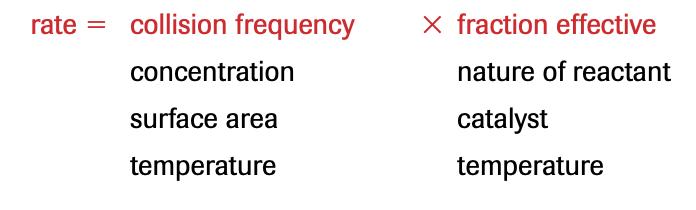
\includegraphics[width=0.6 \textwidth]{../figures/factors-affecting-rate-and-collision-theory.png}
\end{figure}

\begin{figure}[ht!]
    \centering
    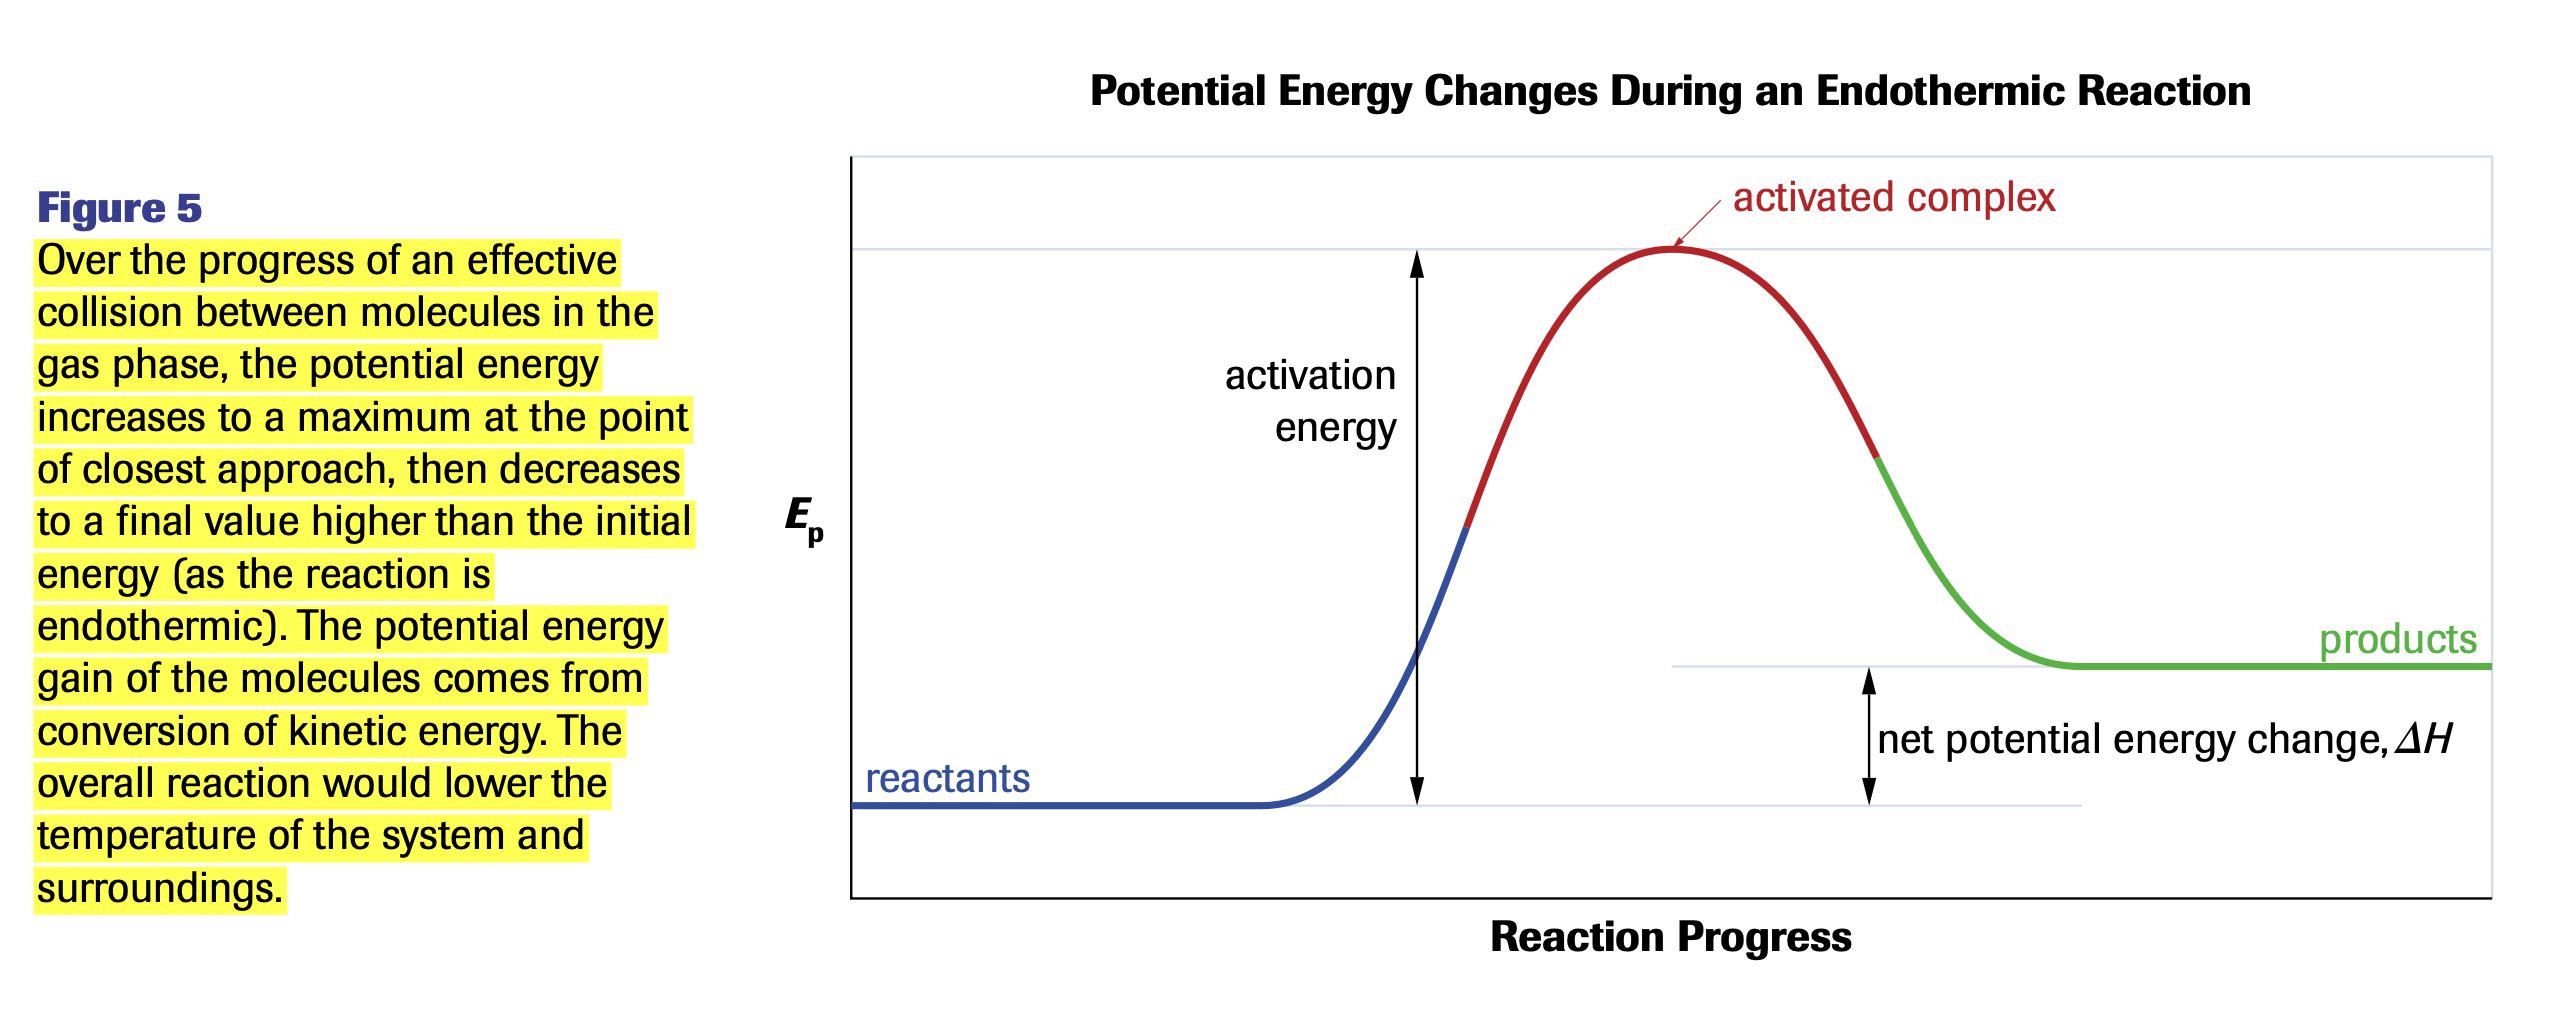
\includegraphics[width=\textwidth]{../figures/endothermic-reaction-curve.png}
\end{figure}

\begin{figure}[ht!]
    \centering
    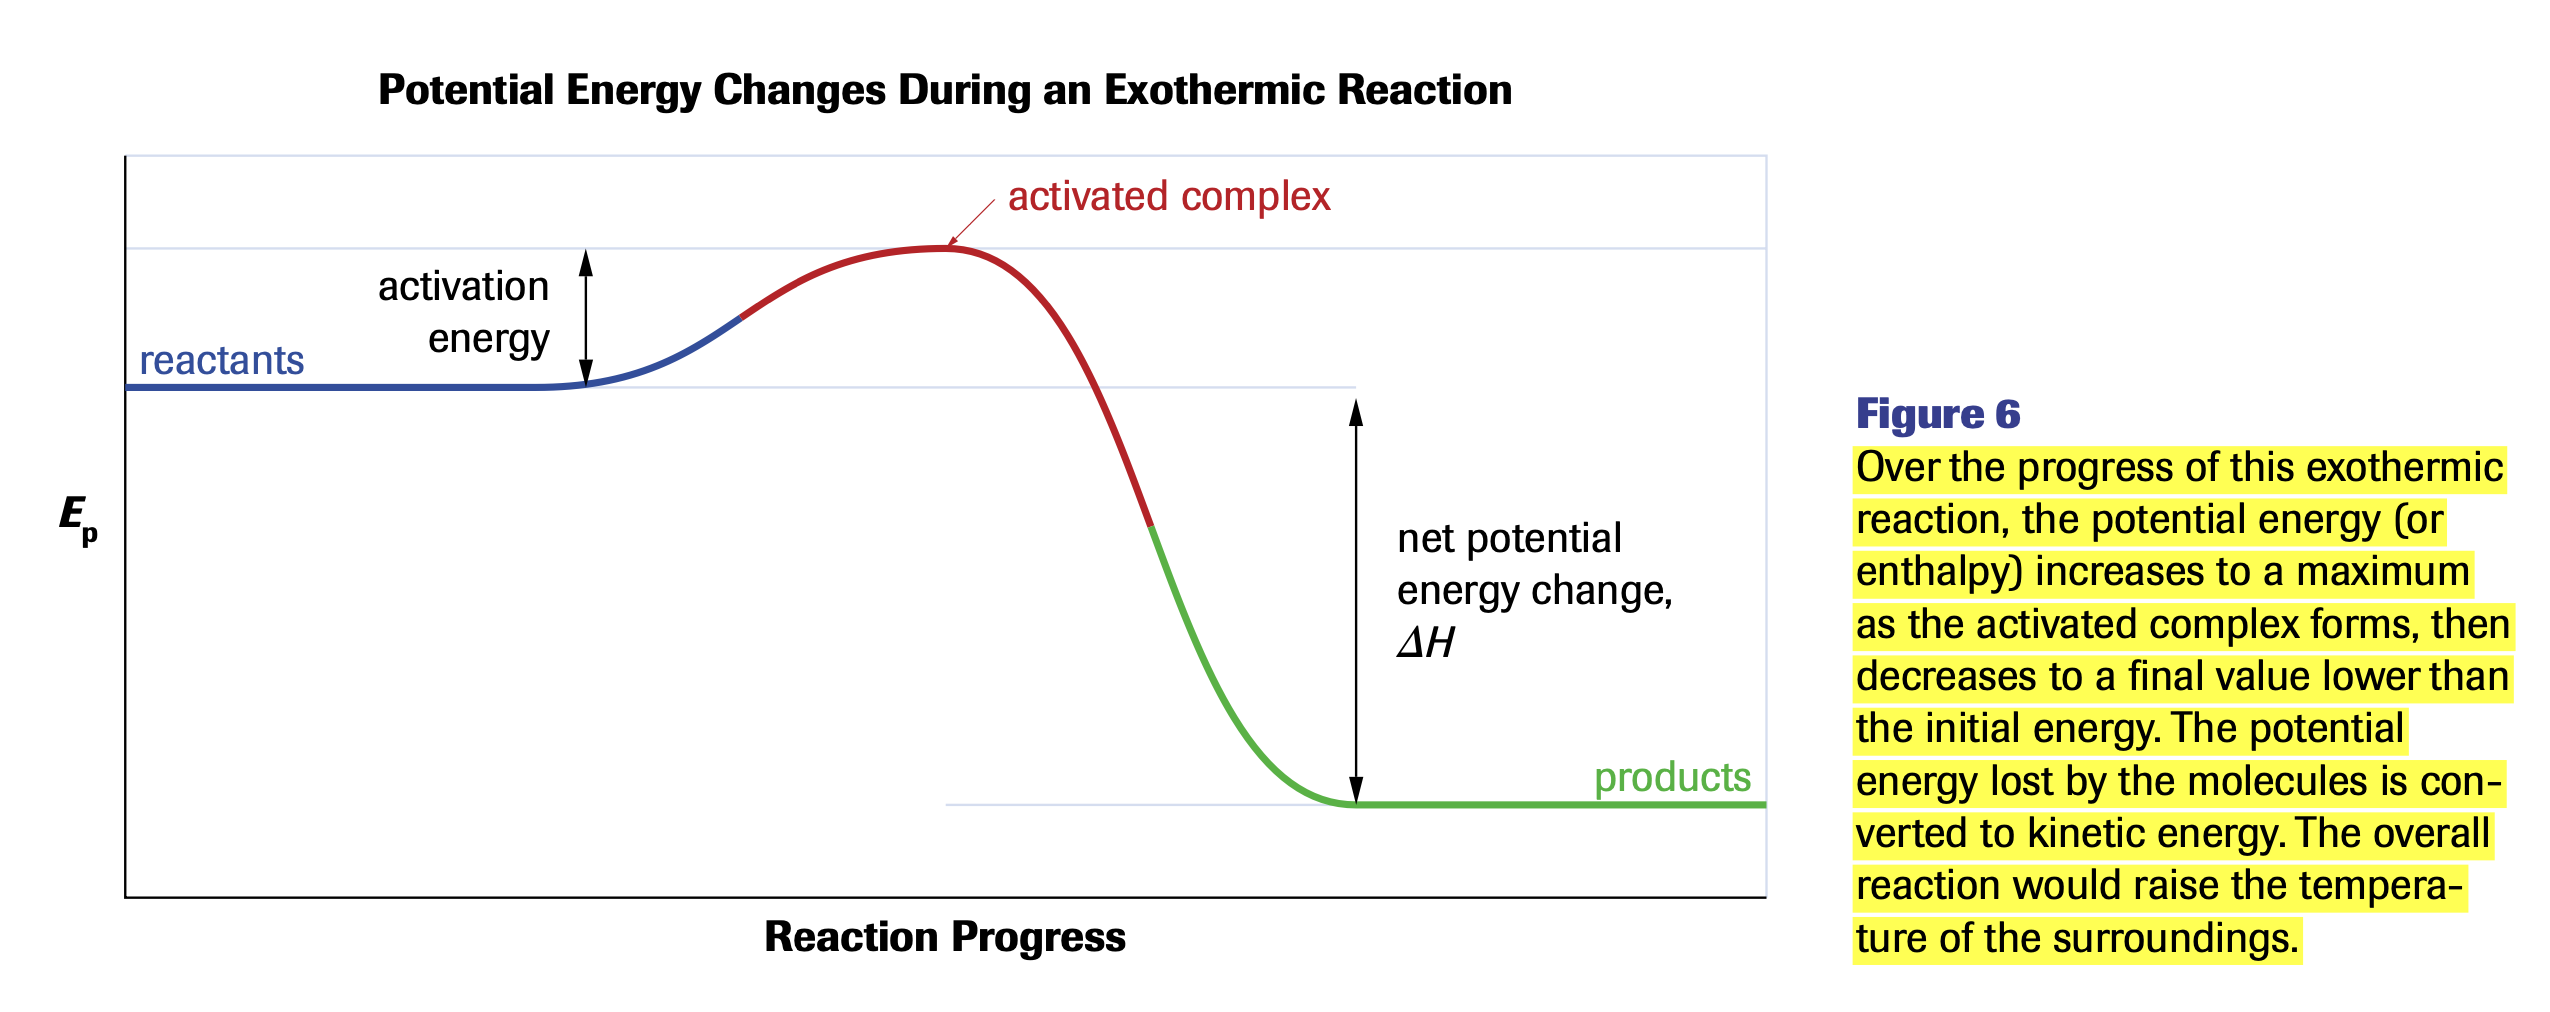
\includegraphics[width= \textwidth]{../figures/exothermic-reaction-curve.png}
\end{figure}

\begin{bulleted-list}
    \item If the molecules have enough kinetic energy, they can approach closely enough for their
        bond structures to rearrange to form an \textbf{activated complex}\footnote{
            \textbf{Activated complex:} an unstable molecule with particular geometry. It is unstable
            because it possesses the maximum potential energy possible. The activated complex
            is also called the \textbf{transition state}.
        }
    \item When the reacting system reaches the activated complex, it may reverse the reaction
        to become the original reactants or form new products
\end{bulleted-list}

\begin{important}
    When the products of a reaction have higher potential energy than the reactants, they will
    have lower kinetic energy (temperature). In their subsequent collisions with other molecules
    in the system, they will tend to decrease the speed of the molecules, resulting in a drop
    in temperature of the system. This is why endothermic reactions reduce the temperature of
    their surroundings.
\end{important}

\subsection{Reaction Mechanisms}
\begin{bulleted-list}
    \item Scientists believe that most chemical reactions occur in a series of \textbf{elementary
        steps}. This overall sequence is called a \textbf{reaction mechanism}
    \item \textbf{Elementary step:} a step in a reaction mechanism that only involves one-, two-,
        or three-particle collisions
    \item \textbf{Reaction mechanism:} a series of elementary steps that make up an overall reaction
\end{bulleted-list}
One good analogy is the Ford automobile production line. Each elementary step can be represented
as a worker, specializing in one part of the manufacturing of an automobile. Furthermore, the
production rate would be most affected by the slowest worker in the production line. Increasing
the concentration at fast steps will have negligible impact on the overall rate, whereas increasing
the concentration at the slowest step will have significant impact.\\

For instance, consider the reaction mechanism of the oxidation of hydrogen bromide
\[
    4 \ch{HBr_{(g)}}+\ch{O2_{(g)}}\to 2\ch{H2O_{(g)}}+2 \ch{Br2_{(g)}}
\]
Which can be represented as a series of reactions
\begin{figure}[ht!]
    \centering
    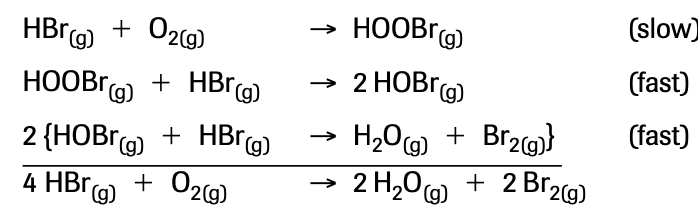
\includegraphics[width=0.5 \textwidth]{../figures/oxidation-of-hydrogen-bromide-reaction-intermediates.png}
\end{figure}

The products, such as HOBr and HOOBr, which are formed but are reacted immediately again to form
new products are called \textbf{reaction intermediates}. 

\begin{figure}[ht!]
    \centering
    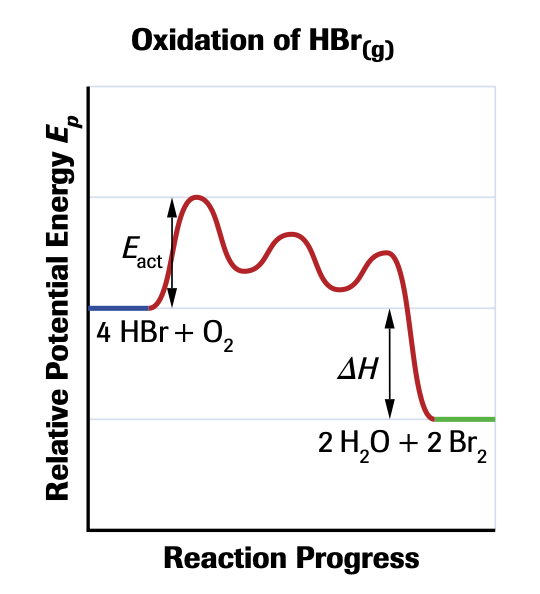
\includegraphics[width=0.6 \textwidth]{../figures/oxidation-of-hydrogen-bromide-graph.png}
    \caption{Keep in mind that the first peak is the reaction intermediate because it requires
    the most substantial increase in energy, and likewise the slowest. Energy released as kinetic
    energy past this point is sufficient to carry out the reaction mechanism.}
    \label{fig:oxidation-of-hydrogen-bromide-graph}
\end{figure}

\begin{important}
    The slowest step in any reaction is called the \textbf{rate-determining step}. \textbf{Reaction
    intermediates} are short-lived products formed in reaction mechanisms.
\end{important}

In general, if the empirically determined rate equation is
\[
    r\propto [X]^n[Y]^m
\]
The rate-determining step in the reaction mechanism must be
\[
    nX+mY\to \text{products or reaction intermediates}
\]
Reaction mechanisms are only ``best guesses'' at the behaviour of molecules, but there are three
rules that must be followed
\begin{enum}
    \item Each step must be elementary; involving no more than three reactants
    \item The slowest rate-determining step must be consistent with the rate equation
    \item The elementary steps must add up to form the overall equation
\end{enum}

\subsection{Theoretical Effect of Chemical Nature of Reactants}
There is a distribution that represents the number of molecules with respect to the kinetic energy.
This distribution is called the \textbf{Maxwell-Boltzmann Distribution}. In a chemical reaction,
an effective collision requires kinetic energy that is converted to potential energy. The minimum
energy is called the \textbf{threshold energy}\footnote{
    \textbf{Threshold energy:} the minimum kinetic energy required to convert kinetic energy to
    activation energy during the formation of the activated complex.
}

\begin{figure}[ht!]
    \centering
    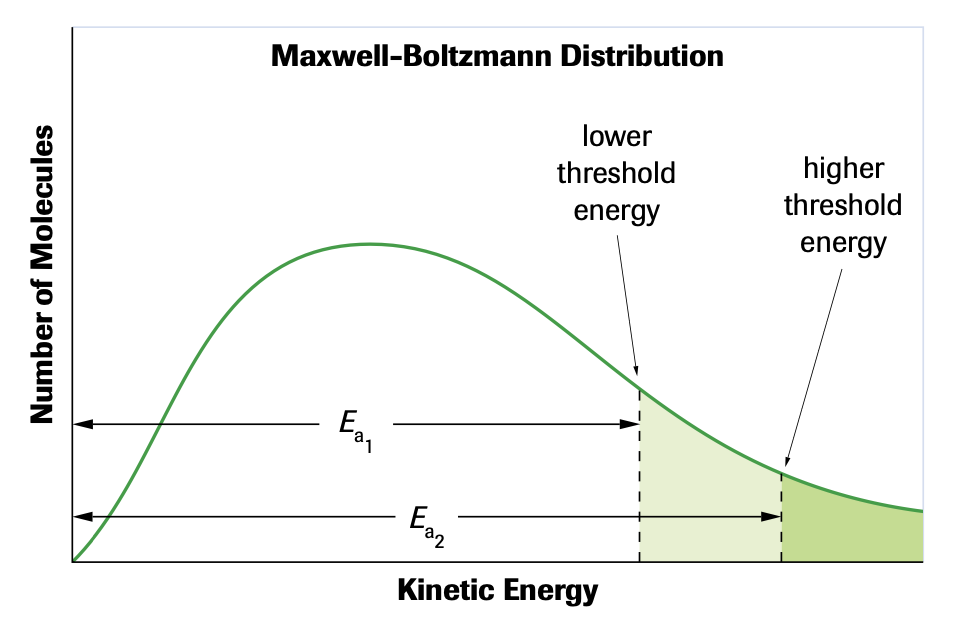
\includegraphics[width=0.8 \textwidth]{../figures/maxwell-boltzmann-distribution.png}
\end{figure}

\begin{sample}{Use collision theory to explain why the permanganate ion ($\ch{MnO4^-}$) reacts much
    more quickly with iron(II) ions ($\ch{Fe}^{2+}$) than with oxolate ions ($\ch{C2O4^{2-}}$)}
    This is because oxolate ions are more complex than permanganate ions, requiring more precise
    collision geometry and a higher activation energy. Thus, the fraction of successful collisions
    is smaller.
\end{sample}

The chemical nature of reactants affects the threshold energy in 2 possible ways:
\begin{enum}
    \item Some molecules have bonds that are relatively weak and small activation energy barriers,
        so the threshold energy is relatively low and a large fraction of them are able to collide effectively
    \item Some molecules have complex geomtry with multiple bonds to be broken, thus requires correct
        orientation when colliding
\end{enum}

\subsection{Theoretical Effect Concentration and Surface Area}
\begin{bulleted-list}
    \item \textbf{Concentration:} generally, as the concentration of a reactant increases, so does
        the reaction rate
    \item \textbf{Surface area:} this only applies to heterogeneous reactions. As surface area
        of the reactants increases, the reaction rate also increases
\end{bulleted-list}

\begin{sample}{Use collision theory to explain why in a flame, a steel wool burns while a steel
    nail just glows.}
    This is because the steel wool has more surface area than the steel nail. Thus, the collision
    frequency is higher.
\end{sample}

\begin{sample}{Use collision theory to explain why liquid nitroglycerin is a dangerous explosion
    but people with heart conditions take nitroglycerin tablets.}
    This is bceause nitroglycerin tablets have a much lower concentration than liquid nitroglycerin.
\end{sample}

\subsection{Theoretical Effect of Temperature}
An increase in temperature has a dramatic effect on the reaction rate, because it increases both
kinetic energy and collision frequency. This equates to a shift in the Maxwell-Boltzmann distribution
curve, where there will be significantly more particles under the curve that are beyond the minimum
threshold energy. 

\subsection{Theoretical Effect of Catalysis}
Theoretically, a catalyst accelerates a reaction by providing an alternative lower energy pathway
from reactants to products. That is, the catalyst allows the reaction to occur through a different
reaction mechanism, with different elementary steps that require less energy. If the new mechanism
has a lower activation energy, a greater fraction of molecules possesses the minimum required
threshold/activation energy (as described by  the Maxwell-Boltzmann distribution curve), and thus 
the reaction rate increases.
